\documentclass[12pt]{article}

\usepackage{graphicx}
\usepackage{caption}
\usepackage{amsmath, amssymb, amsthm}
\usepackage{booktabs}
\usepackage{enumitem}
\usepackage{geometry}
\geometry{margin=1in}
\usepackage{xcolor}
\usepackage{float}
\usepackage{tabularx}
\usepackage[normalem]{ulem} % normalem keeps \emph working normally
\usepackage{algorithm}
\usepackage{algpseudocode}
\usepackage[colorlinks=true, allcolors=blue]{hyperref} % load near the end
\usepackage[capitalise]{cleveref} % must be loaded after hyperref

\title{NPSC3000 End of Year Report: Can Reinforcement Learning Outperform Traditional Methods for Cloud Resource Allocation}
\author{
\textbf{Student:} Ty Riekert \\
\textbf{Supervisor:} Elham Mardaneh \\
\textbf{Co-supervisor:} Tony Mathew
}
\date{Sept 2026}

\begin{document}
\maketitle
\begin{abstract}
The problem of resource allocation (RA) is a critical issue amongst cloud providers \cite{saidi2023, sdn2021, vinothina2012, parikh2013, mohamaddiah2014}. Consider a shared pool of physical servers that must serve a continuous stream of user jobs while meeting a variety of metrics like meeting deadlines, reducing tardiness and limiting energy usage. Classical scheduling methods are known to struggle with the dynamic, multi-objective nature of this problem \cite{lbts2024, 10854610, DAHMANI2025100616}, while reinforcement learning (RL) has held promising results in similar settings \cite{saidi2023, autoscaling2023, lbts2024, dynamic2026}. This project asks \textbf{under which conditions and objectives does RL outperform classical scheduling methods}. We model this cloud RA problem as a resource-constrained scheduling optimisation problem in two settings: offline, where all jobs are known in advance, and online, where jobs arrive randomly throughout some time period. We consider a multitude of RL design decisions on proximal policy optimisation (PPO) and advantage actor-critic (A2C) RL algorithms against 49 heuristic combinations and the CP-SAT exact solver. On the main objective (\cref{eq:objective-v2}), optimising for only weighted squared tardiness, the best RL agent is 5\% behind the best heuristic offline. When the objective also counts linear tardiness or the number of late jobs, RL outperforms the best heuristic by 2--10\% offline. Online, RL is more sensitive to training budget and seed: increasing training from 300k to 1M steps improved results substantially, and the best seed at 1M steps comes within 4\% of the best heuristic, although the mean over seeds remains 21\% behind. Overall, RL is most competitive when the objective combines several metrics, but struggles in the online scenario, where training increases in complexity substantially.
\end{abstract}

\newpage
\section{Project Aims and Deliverables}
The aim of this project is to formulate cloud resource allocation as a mathematical optimisation and reinforcement learning problem, and to implement and rigorously evaluate RL models against established methods. The specific deliverables are:
\begin{itemize}
    \item Conduct comprehensive research on current findings and machine learning in cloud resource allocation
    \item Formulate a mathematical model of the cloud RA problem, expressed as a resource-constrained scheduling optimisation problem
    \item Create a corresponding Markov Decision Process (MDP) formulation for the reinforcement learning agent
    \item Implement the code of the scheduling environment
    \item Implement the code for the reinforcement learning agent(s)
    \item Evaluate the trained agents against classical scheduling heuristics to determine under what conditions reinforcement learning outperforms traditional methods.
\end{itemize}
The last item is not done with a single `train and compare' run, but is an iterative process repeated throughout the second half of the project: a constant loop of training, evaluating against baselines, examining and researching behaviour and faults, and revising.

\section{Background}
\subsection{Cloud Computing}
Cloud computing refers to the use of computing services and resources delivered over the internet, and resource allocation (RA) is one of the most critical challenges facing cloud providers today \cite{saidi2023, huawei2022}. As cloud infrastructure underpins the majority of modern computing services, effectively allocating physical resources, like compute or network bandwidth, to a continuously arriving stream of workloads has become of vital importance to providers \cite{sdn2021}. Poor allocation leads to poor metrics in response time, environmental sustainability, energy or power efficiency, throughput, makespan, utilisation and more \cite{cloudkpi2010, dvbpp2026, mohamaddiah2014, anuradha2014}.

\subsubsection{Cloud RA}
Cloud RA can be decomposed into several coupled problems. Virtual machine (VM) placement decides which physical server hosts each virtual machine, subject to resource constraints like CPU and memory. This is widely regarded as the core RA subproblem \cite{saidi2023}. Task scheduling decides when and on which resource each user task should run, and considers metrics such as execution time, response time or deadline of work \cite{lbts2024}. Autoscaling dynamically adjusts resource capacity to match fluctuating demand in real time \cite{autoscaling2023}, and load balancing distributes incoming tasks evenly to avoid hotspots \cite{lb2024}.

Solutions to these problems generally fall into three categories:
\begin{itemize}
    \item \textbf{Exact Methods.} Algorithms that always solve a problem optimally.
    \item \textbf{Approximation Methods.} These methods are used when exact algorithms become computationally infeasible. Two main classes are heuristics, problem-specific rules designed to quickly construct or improve a single solution, and metaheuristics, general-purpose strategies that can guide heuristic methods \cite{alkhalifa2025comparative}.
    \item \textbf{Machine learning.} Methods that learn decision rules from data instead of manually from people.
\end{itemize}

Exact methods guarantee optimality on small instances, scale terribly, and in practice are limited to providing best-solution bounds. Heuristics and metaheuristics scale well, but can yield approximate solutions that may not be sufficiently accurate. Systematic reviews within this field identify five major problems of these approximation methods: scalability, adaptability, multi-objective complexity, high computational cost with scale, and real-time decision making \cite{mohamaddiah2014, lbts2024, 10854610, DAHMANI2025100616, ml_ra_litrev2025, hu2021attend2pack}.

\subsubsection{Motivations for Machine Learning}
The above-mentioned limitations motivate a growing body of work applying machine learning, and reinforcement learning specifically, to combinatorial and scheduling problems. A fixed heuristic relies on designer intuition to determine what makes a job important and applies that rule unchanged through deployment. RL still requires design choices, such as what it should optimise for, but the policy for assigning jobs to machines is learnt during training, in an environment that should reflect the deployment environment \cite{ml_ra_litrev2025}. Systematic reviews of RL for scheduling or bin packing report encouraging growth in this area \cite{DAHMANI2025100616}, and prior systems like DeepRM \cite{mao2016deeprm} and Decima \cite{mao2019decima} showed learned schedulers matching or exceeding hand-designed rules on cluster workloads.

This project examines two actor-critic RL methods, Proximal Policy Optimisation (PPO) and Advantage Actor-Critic (A2C), the synchronous version of A3C \cite{schulman2017ppo, mnih2016a3c, apxml_a2c_a3c_2026, aigreeksActorCritic, chadia2023understandingRL, konda1999actorcritic}. We also examine variations like hyper-heuristics \cite{burke2013hyperheuristicsurvey, lassoued2026hyperheuristic, cie2025dispatchruleselection} and hybrid RL designs \cite{min2022atctuning, chen2024drlgphh}. These learning algorithms are then placed against classical dispatching heuristics \cite{vepsalainen1987atc}, a metaheuristic and an exact solver \cite{ortools}.

\subsubsection{Project Motivation}
RL for cloud RA is in active research \cite{ml_ra_litrev2025, DAHMANI2025100616}, but existing papers mainly review only a few objectives for RL, and compare against a limited set of baselines. Most model the problem as bin packing or VM placement, and few focus on a multi-objective resource-constrained scheduling view \cite{cloud_rco}. We would like to see:
\begin{center}
\textbf{Under which objectives and conditions does RL outperform classical scheduling algorithms on the problem of cloud RA?}
\end{center}

\subsubsection{Markov Decision Process}\label{sec:MDP_ssSection}
The Markov Decision Process (MDP) is a foundational framework for decision making in stochastic and uncertain environments \cite{DRL_Intrusion}. It is the core structure used for an RL program. At any time $t$ it has a state $s_t$ that reflects the current state of the environment, and the actions available $a_t$ (often masked to get rid of infeasible actions \cite{huang2020invalidmasking}). The agent chooses an action $a_t$, and the environment moves from state $s_t$ to $s_{t+1}$.

An MDP is described as a tuple $(S, A, P, R, \gamma)$. We have the sets $S$ (state space) and $A$ (action space). $P$ is the transition probability that satisfies the Markov property,
\begin{equation}\label{Markov_Property}
    p(s_{t+1} \mid s_1, a_1, s_2, a_2, \dots, s_t, a_t) = p(s_{t+1} \mid s_t, a_t).
\end{equation}
$p(s' \mid s, a) \in P$ describes the probability of transferring to a specific state $s'$ by taking action $a$ in the given state $s$. The reward function $R : S \times A \rightarrow \mathbb{R}$ gives the expected immediate reward $R(s, a) = \mathbb{E}[r_t \mid s_t = s, a_t = a]$ that the agent receives after taking action $a$ in state $s$. Finally, $\gamma \in (0, 1]$ is the discount factor that can be used to indicate short-term or long-term importance of rewards. The MDP loop can be seen in \cref{fig:MDP_Diagram}. The final goal of an agent in an MDP is to maximise the overall reward.
\begin{figure}[htbp]
    \centering
    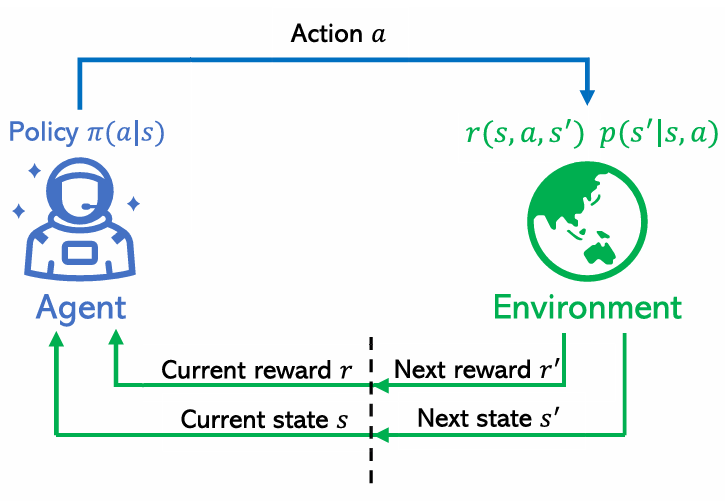
\includegraphics[width=0.5\linewidth]{Images/MDP_Diagram.png}
    \caption{Agent Interaction With MDP}
    \label{fig:MDP_Diagram}
\end{figure}

\subsection{Reinforcement Learning}\label{sec:rl}
RL is a decision-making computer program that starts with no prior knowledge, and learns to make decisions from repeated interactions with an environment, using the reward for its decisions as feedback \cite{LADOSZ20221}. The problem is formalised as a Markov Decision Process (MDP) (\cref{sec:MDP_ssSection}) \cite{LADOSZ20221, DRL_Intrusion}. The agent learns a policy: a probability distribution over actions $a_t$ for a given state $s_t$, chosen to maximise the expected total reward.

RL methods fall into two main families. \textbf{Value-based} methods learn the expected return of each action and greedily choose the action with the highest return. \textbf{Policy-gradient} methods directly adjust the policy parameters towards a higher return \cite{williams1992reinforce}. \textbf{Actor-critic} methods combine the two: a critic (a value function) learns the expected return from each state, and the actor (a policy-gradient method) uses the critic's estimates to judge how good a decision was and guide its updating of the policy \cite{konda1999actorcritic}.

\section{Methodology}
\subsection{Problem Formulation}\label{sec:problem}
A cloud computing environment receives a set of jobs that need to be assigned to a set of physical machines. Each job $j$ has a fixed processing duration $p_j$, a fixed multi-dimensional vector of resource requirements $a_{jr}$ (e.g.\ CPU, memory) which it occupies for its entire duration, and a due date $d_j$ by which the job should be completed. Jobs are assumed to be independent of one another. To reflect that some jobs matter more than others, each job is given a priority weight $w_j$, which we assume is set externally according to business needs.

Jobs are served by a set of identical machines $M$, each limited only by a fixed capacity $C_r$. A machine may process several jobs simultaneously, provided their combined resource usage does not exceed its capacity in any dimension. We model the scheduling to be non-preemptive: each job is assigned to exactly one machine at a single start time, and runs uninterrupted until completion. We discretise time into integer steps over a finite planning horizon $H$. The tardiness of a job $j$ is then
\begin{equation}\label{eq:tardiness}
    T_j = \max\left(0,\; s_j + p_j - d_j\right),
\end{equation}
and $U_j = 1$ if job $j$ finishes late. Notation is summarised in Appendix~\ref{sec:AppendixA}, and the full constraint set in Appendix~\ref{sec:AppendixB}.

\subsection{Objective Function}\label{sec:objectives}
The first objective considered the number of machines used, weighted tardiness, and peak utilisation $\theta$,
\begin{equation}\label{eq:objective-v1}
    \min \; \lambda_1 \sum_{m \in M} y_m \;+\; \lambda_2 \sum_{j \in J} w_j T_j \;+\; \lambda_3\, \theta.
\end{equation}
Experiments under \cref{eq:objective-v1} found it could be gamed and hacked \cite{skalse2022rewardhacking}: unscheduled jobs incurred no loss, the machine activation penalty provided no real input (a once-off penalty), and the peak-utilisation term worked against energy-efficient consolidation \cite{energyaware2012, fan2007powerprovisioning}. It was replaced by a weighted sum of optional metrics:
\begin{equation}\label{eq:objective-v2}
    \min \; J_{\lambda} = \underbrace{\sum_{j} w_j T_j^{2}}_{J}
          \;+\; \lambda_T \sum_{j} w_j T_j
          \;+\; \lambda_U \sum_{j} w_j U_j
          \;+\; \lambda_E E,
\end{equation}
covering squared tardiness, linear tardiness, the weighted number of late jobs, and energy (measured as total active machine-time \cite{fan2007powerprovisioning}), respectively. The main objective of this project was squared tardiness alone ($J$), penalising a few very late jobs more than many slightly late jobs. At the end of the scheduling horizon, instead of ending the episode, jobs continue to be placed and accumulate tardiness until completion. This way, leaving a job unscheduled is always costly, removing the loophole the original objective had. The other metrics in this new objective are only considered in the multi-objective experiments.

\subsection{Offline and Online Cases}\label{sec:cases}
We would like to study two cases of the problem: offline, when all jobs are known and available at $t = 0$ but only a single job can be assigned at each time index, and online, where jobs arrive (are revealed) over time through a Poisson process \cite{kleinrock1975queueing, mao2016deeprm} but multiple jobs can be assigned at any given time step.

The difficulty of the online case is set by the load factor $\rho$, which measures how busy the cluster is on average. A job $j$ brings $p_j a_{jr}$ units of work. Jobs arrive at rate $\nu$ per time step, so on average $\nu\,\mathbb{E}[p_j a_{jr}]$ units of work arrive per time step, while the cluster can process at most $|M|\, C_r$ units per time step. Their ratio is the utilisation, and taking the largest ratio over the resources gives the bottleneck,
\begin{equation}\label{eq:rho}
    \rho = \max_{r \in R} \frac{\nu\, \mathbb{E}[p_j a_{jr}]}{|M|\, C_r}.
\end{equation}
Work consequently accumulates when $\rho \ge 1$. Loads from $\rho = 0.50$ to $1.10$ are studied, with log-normal job sizes matching the right-skewed distributions of real cluster traces \cite{reiss2012googletrace, cortez2017resourcecentral}.

\subsection{Markov Decision Process}\label{sec:mdp}
To formulate this problem for our algorithms, we use a Markov Decision Process $(S, A, P, R, \gamma)$ as discussed in \cref{sec:MDP_ssSection}.

\paragraph{State $S$.} We define the state to hold each currently waiting job's ($j \in J_t \subseteq J$) features $F_j = (p_j, a_j, d_j, w_j)$, along with each currently processing job, where a job enters the processing set $P_t \subseteq J$ when it gets assigned. For each processing job, we instead hold $G_j = (m_j, s_j, p_j)$: which machine the job is assigned to, its start time and its total duration. On top of the jobs, we include the remaining capacity of each machine,
\begin{equation}\label{eq:remaining-capacity}
    R_{mrt} = C_r - \sum_{j \in P_t:\ m_j = m} a_{jr},
\end{equation}
and $y = (y_m)_{m \in M}$ to record which machines are switched on. This yields a state vector,
\begin{equation}\label{eq:state}
    s_t = \big(J_t,\ P_t,\ \{F_j\}_{j \in J_t},\ \{G_j\}_{j \in P_t},\ \{R_{mrt}\}_{m \in M,\, r \in R},\ y,\ t\big).
\end{equation}

\paragraph{Action space $A$.} At each step, the agent can assign waiting jobs to machines, and/or idle,
\begin{equation}\label{eq:action-flat}
    A_t = \{(j, m) : j \in J_t,\ m \in M\} \cup \{\text{idle}\}.
\end{equation}
For the offline case, an agent can only produce a single action at each time step. For the online case, an agent can continuously take actions at the same step $t$, only progressing to the next time step when it decides to idle.

\paragraph{Transition dynamics $P$.} An assignment action $(j, m)$ moves job $j$ from $J_t$ to $P_t$ with $s_j = t$ and $m_j = m$, activating machine $m$ if needed. When time advances (after every action offline, and only after an idle online), completed jobs leave the processing set by \cref{eq:processing-update}, their capacity is released, and online, newly arrived jobs join $J_{t+1}$. Transitions are deterministic offline, and stochastic online only through arrivals.
\begin{equation}\label{eq:processing-update}
    P_{t+1} = \{k \in P_t : s_k + p_k > t + 1\}.
\end{equation}

\paragraph{Reward $R$.} The reward is the negative of $J$, charged as tardiness accrues, plus a potential-based shaping term that provably leaves the optimal policy unchanged \cite{ng1999shaping}.

\subsection{Methods Compared}\label{sec:baselines}
In this project, a variety of algorithms are examined, grouped into four categories. We summarise these algorithms as follows.

\subsubsection{Learning Algorithms}\label{sec:algorithms}
\paragraph{Reinforcement Learning.} All RL policy methods examined are actor-critic methods: A2C and PPO, chosen for their robustness and simplicity. We consider these algorithms under several action-space designs:
\begin{itemize}
    \item \textbf{Option 0 -- Direct Job-Machine Selection:} The policy picks a (job, machine) pair with a pointer-network architecture \cite{vinyals2015pointernet, kool2019attention}. A large discrete action space is a known struggle for policy-gradient methods.
    \item \textbf{Option 1 -- Hyper-heuristic Rule Selection:} The policy chooses which dispatching rule to apply at each decision \cite{burke2013hyperheuristicsurvey, lassoued2026hyperheuristic}.
    \item \textbf{Option 2 -- Priority Learning:} The policy picks which job to start next, learning its own priority from the job features; a fixed First-Fit rule then places it, making this a hybrid of RL and a dispatching heuristic.
    \item \textbf{Option 3 -- Priority Learning with ATC:} Option 2 with the ATC index \cite{vepsalainen1987atc} as an extra feature; Option 3w is restricted to the 20 most urgent jobs \cite{mao2016deeprm}.
    \item \textbf{Option 4 -- Action Branching:} The job and machine are chosen by two separate heads instead of together (flat) \cite{tavakoli2018actionbranching}.
\end{itemize}
Moreover, variants of the two RL algorithms, Reward Constrained Policy Optimisation (RCPO) for a different reward function approach, and PPO-Lagrangian, were also examined.

\subsubsection{Baseline Algorithms}
\paragraph{Dispatching Heuristics.} Each heuristic combines a priority rule to choose the next job, and a placement rule to choose the next machine.
\begin{itemize}
    \item \textbf{Priority Rules:} Earliest Deadline First (EDF) and Least Slack Time (LST), which prioritise urgency; Shortest and Longest Processing Time (SPT, LPT); Weighted SPT (WSPT) \cite{smith1956wspt}; First-Come-First-Served (FCFS, also known as FIFO); the Apparent Tardiness Cost (ATC) rule, balancing job weight, length and urgency \cite{vepsalainen1987atc}; WMDD \cite{kanet2004wmdd} and COVERT \cite{carroll1965covert}. Three weighted rules were also built for this project after the first RL results: WLST and WEDF, which scale a job's slack by its weight, and MDC, which applies Smith's ratio rule \cite{smith1956wspt} to the marginal increase in squared tardiness.
    \item \textbf{Placement Rules:} First-Fit, Best-Fit, Worst-Fit, and Consolidate, a more energy-aware approach \cite{energyaware2012}.
    \item \textbf{Tetris:} A multi-resource packing heuristic scoring job-machine pairs jointly \cite{grandl2014tetris}.
\end{itemize}
This gives 49 heuristics in total.

\paragraph{Metaheuristic.} Particle Swarm Optimisation (PSO) \cite{kennedy1995pso}, in which each particle encodes a job ordering decoded into a schedule, was tested earlier in the project but was always worse than the best rule, so it is not part of the final comparison.

\paragraph{Exact Solver.} CP-SAT \cite{ortools}, a constraint-programming solver, models the scheduling problem exactly. Given 60 seconds per instance, it returns the best schedule it has found, an upper bound on the optimum, together with a proven lower bound.

\subsection{Implementation}\label{sec:implementation}
The environment, agents and evaluation pipeline are implemented in Python\footnote{\url{https://github.com/Ethan-Ty-Riekert/Neural-Knapsack-Research-Project}} using Gymnasium and Stable-Baselines3 \cite{raffin2021sb3}. The original environment and mathematical formulation were implemented in code manually, with all model implementations, training and evaluation done with Claude Code (see the Generative AI Use Statement).

\subsubsection{Experimental Setup}\label{sec:setup}
\paragraph{Offline} instances have 100 jobs, 10 machines, 4 resources with $C_r = 30$, $H = 100$. Job durations and demands are drawn uniformly from $\{1, \dots, 9\}$, and job weights from $\{1, \dots, 5\}$, with deadlines of medium tightness ($\mathrm{TF} = 0.5$, where TF is the tardiness factor affecting deadline tightness) \cite{potts1985wtardiness}. A matching preset with all $w_j = 1$ is generated to isolate the effects of considering weights.

\paragraph{Online} instances use the same setup (always with weighted jobs), with the addition of Poisson arrivals over $[0, H)$ at loads $\rho \in \{0.50, 0.75, 0.95, 1.10\}$ and deadline slack drawn between 10 and 60. Moreover, job resource sizes are log-normal, mean-matched to the offline distribution. RL was trained and evaluated only offline at TF $= 0.5$ and online at $\rho = 0.95$; the other settings were run for heuristics only.

\paragraph{Training and tuning.} An agent learns over episodes, each a complete, newly generated problem instance, so it never trains on the same problem twice. Training, validation (20 instances) and test (50 instances) use disjoint random seeds, so test instances are never seen in training or tuning. Every combination of design (6), algorithm (2) and case (2) had its own hyperparameter search, 24 studies in all, run with the same protocol: Optuna \cite{akiba2019optuna} with the TPE sampler \cite{bergstra2011tpe}, 12 trials of 300,000 steps, the first trial always being the library defaults. Poor trials were stopped early by median pruning, which compares a trial's validation $J$ with the median of earlier trials \emph{at the same training step}. Each study keeps one best configuration, chosen on the 20 validation instances. That configuration was then retrained with 3 random seeds for 1,000,000 steps offline and 300,000 steps online, and results are the mean and standard deviation over the seeds. A follow-up trained online Options 0, 2 and 3 (PPO) for 1,000,000 steps, and Option 2 for 2,000,000 (Appendices~\ref{sec:AppendixC} and~\ref{sec:AppendixD}).

\paragraph{Evaluation.}\label{sec:evaluation} Every method, RL and baseline, is evaluated on the same 50 held-out test instances for each setting. RL agents act deterministically using a two-stage rule: idle if the probability of idling is at least the total probability of all job actions, otherwise take the most likely job action. We report mean $J$ over the test instances; for RL this is averaged over the 3 seeds, with the standard deviation across seeds. The heuristics are deterministic, so they were run once, with their standard deviation across instances.

We also record metrics that were not optimised, such as the on-time rate, number of late jobs, maximum tardiness and energy. Any pattern in these is a side effect of optimising $J$ rather than a learned trade-off, so it is interpreted with caution.

\paragraph{Multi-objective experiments.}\label{sec:mo-method} To test whether RL's relative performance depends on the objective, every method was also scored on composite objectives $J_\lambda$ (\cref{eq:objective-v2}). The weights $\lambda_T, \lambda_U, \lambda_E$ are set separately for each setting, so that each added term equals $J$ on the best heuristic's schedule; this prevents any term from dominating merely because of its units. Each weight is then multiplied by 0.25, 0.5, 1, 2 and 4. In addition to the agents trained on $J$ alone, Option 2 and 3 PPO agents were trained directly on several composite objectives (300,000 steps offline with default hyperparameters, 3 seeds; 1,000,000 steps online).

\section{Results}\label{sec:results}
All results below are from the evaluation on the 50 held-out instances; lower $J$ is better. Full tables for every setting and metric are on the project's GitHub \href{https://github.com/Ethan-Ty-Riekert/Neural-Knapsack-Research-Project/tree/main/Results}{results page}, and an AI-made interactive atlas (a collection of all results in an HTML page) is \href{https://github.com/Ethan-Ty-Riekert/Neural-Knapsack-Research-Project/tree/main/Results}{here}. % TODO (Ty): replace with the atlas link

\subsection{RL against Heuristics on the Main Objective}\label{sec:res-main}
\Cref{tab:main} and \cref{fig:offline} summarise the main comparison. Looking at the offline case, with weighted jobs the best RL agent (Option 2, PPO) reaches $J = 28{,}061$, 5.2\% above the best heuristic, WLST ($26{,}670$). RL's standard deviation across seeds is small. When every job has the same weight, the problem is much easier for heuristics. LST scores $13{,}098$, and the best RL agents either reproduce it exactly by simply choosing that heuristic (Option 1), or come within 0.8\% (Option 2).

For the online case, RL was only trained at $\rho = 0.95$, and every RL design was far behind the best heuristic: EDF+Consolidate reached $21{,}986$, and the best RL agent (Option 1, A2C), which can choose that same heuristic (i.e.\ we would expect it to match the best heuristic's score exactly), got $37{,}812$ (+72\%). This online gap could be a training-budget issue.

\begin{table}[htbp]
\centering
\caption{Mean $J$ on 50 test instances (lower is better). RL: mean $\pm$ standard deviation over 3 seeds, best algorithm per design; heuristics are deterministic. Online RL is shown at the standard 300k-step budget.}
\label{tab:main}
\begin{tabular}{lrrr}
\toprule
Method & Offline, weighted & Offline, $w_j = 1$ & Online, $\rho = 0.95$ \\
\midrule
Best heuristic & 26,670 (WLST) & 13,098 (LST) & 21,986 (EDF+Cons.) \\
LST+FirstFit & 39,536 & 13,098 & 38,831 \\
EDF+FirstFit & 41,302 & 13,757 & 40,381 \\
CP-SAT (60 s) & 35,681 & 16,469 & -- \\
\midrule
Option 0 (job--machine pairs) & 29,696 $\pm$ 833 & 13,494 $\pm$ 276 & 44,920 $\pm$ 0 \\
Option 1 (rule selection) & 38,645 $\pm$ 142 & 13,098 $\pm$ 0 & 37,812 $\pm$ 8,893 \\
Option 2 (priority) & \textbf{28,061 $\pm$ 219} & 13,207 $\pm$ 28 & 39,947 $\pm$ 11,949 \\
Option 3 (priority + ATC) & 28,282 $\pm$ 537 & 13,496 $\pm$ 98 & 44,827 $\pm$ 2,890 \\
Option 4 (action branching) & 28,577 $\pm$ 43 & 13,411 $\pm$ 181 & 139,721 $\pm$ 101,396 \\
\midrule
Best RL vs best heuristic & +5.2\% & 0.0\% & +72\% \\
\bottomrule
\end{tabular}
\end{table}

\begin{figure}[htbp]
\centering
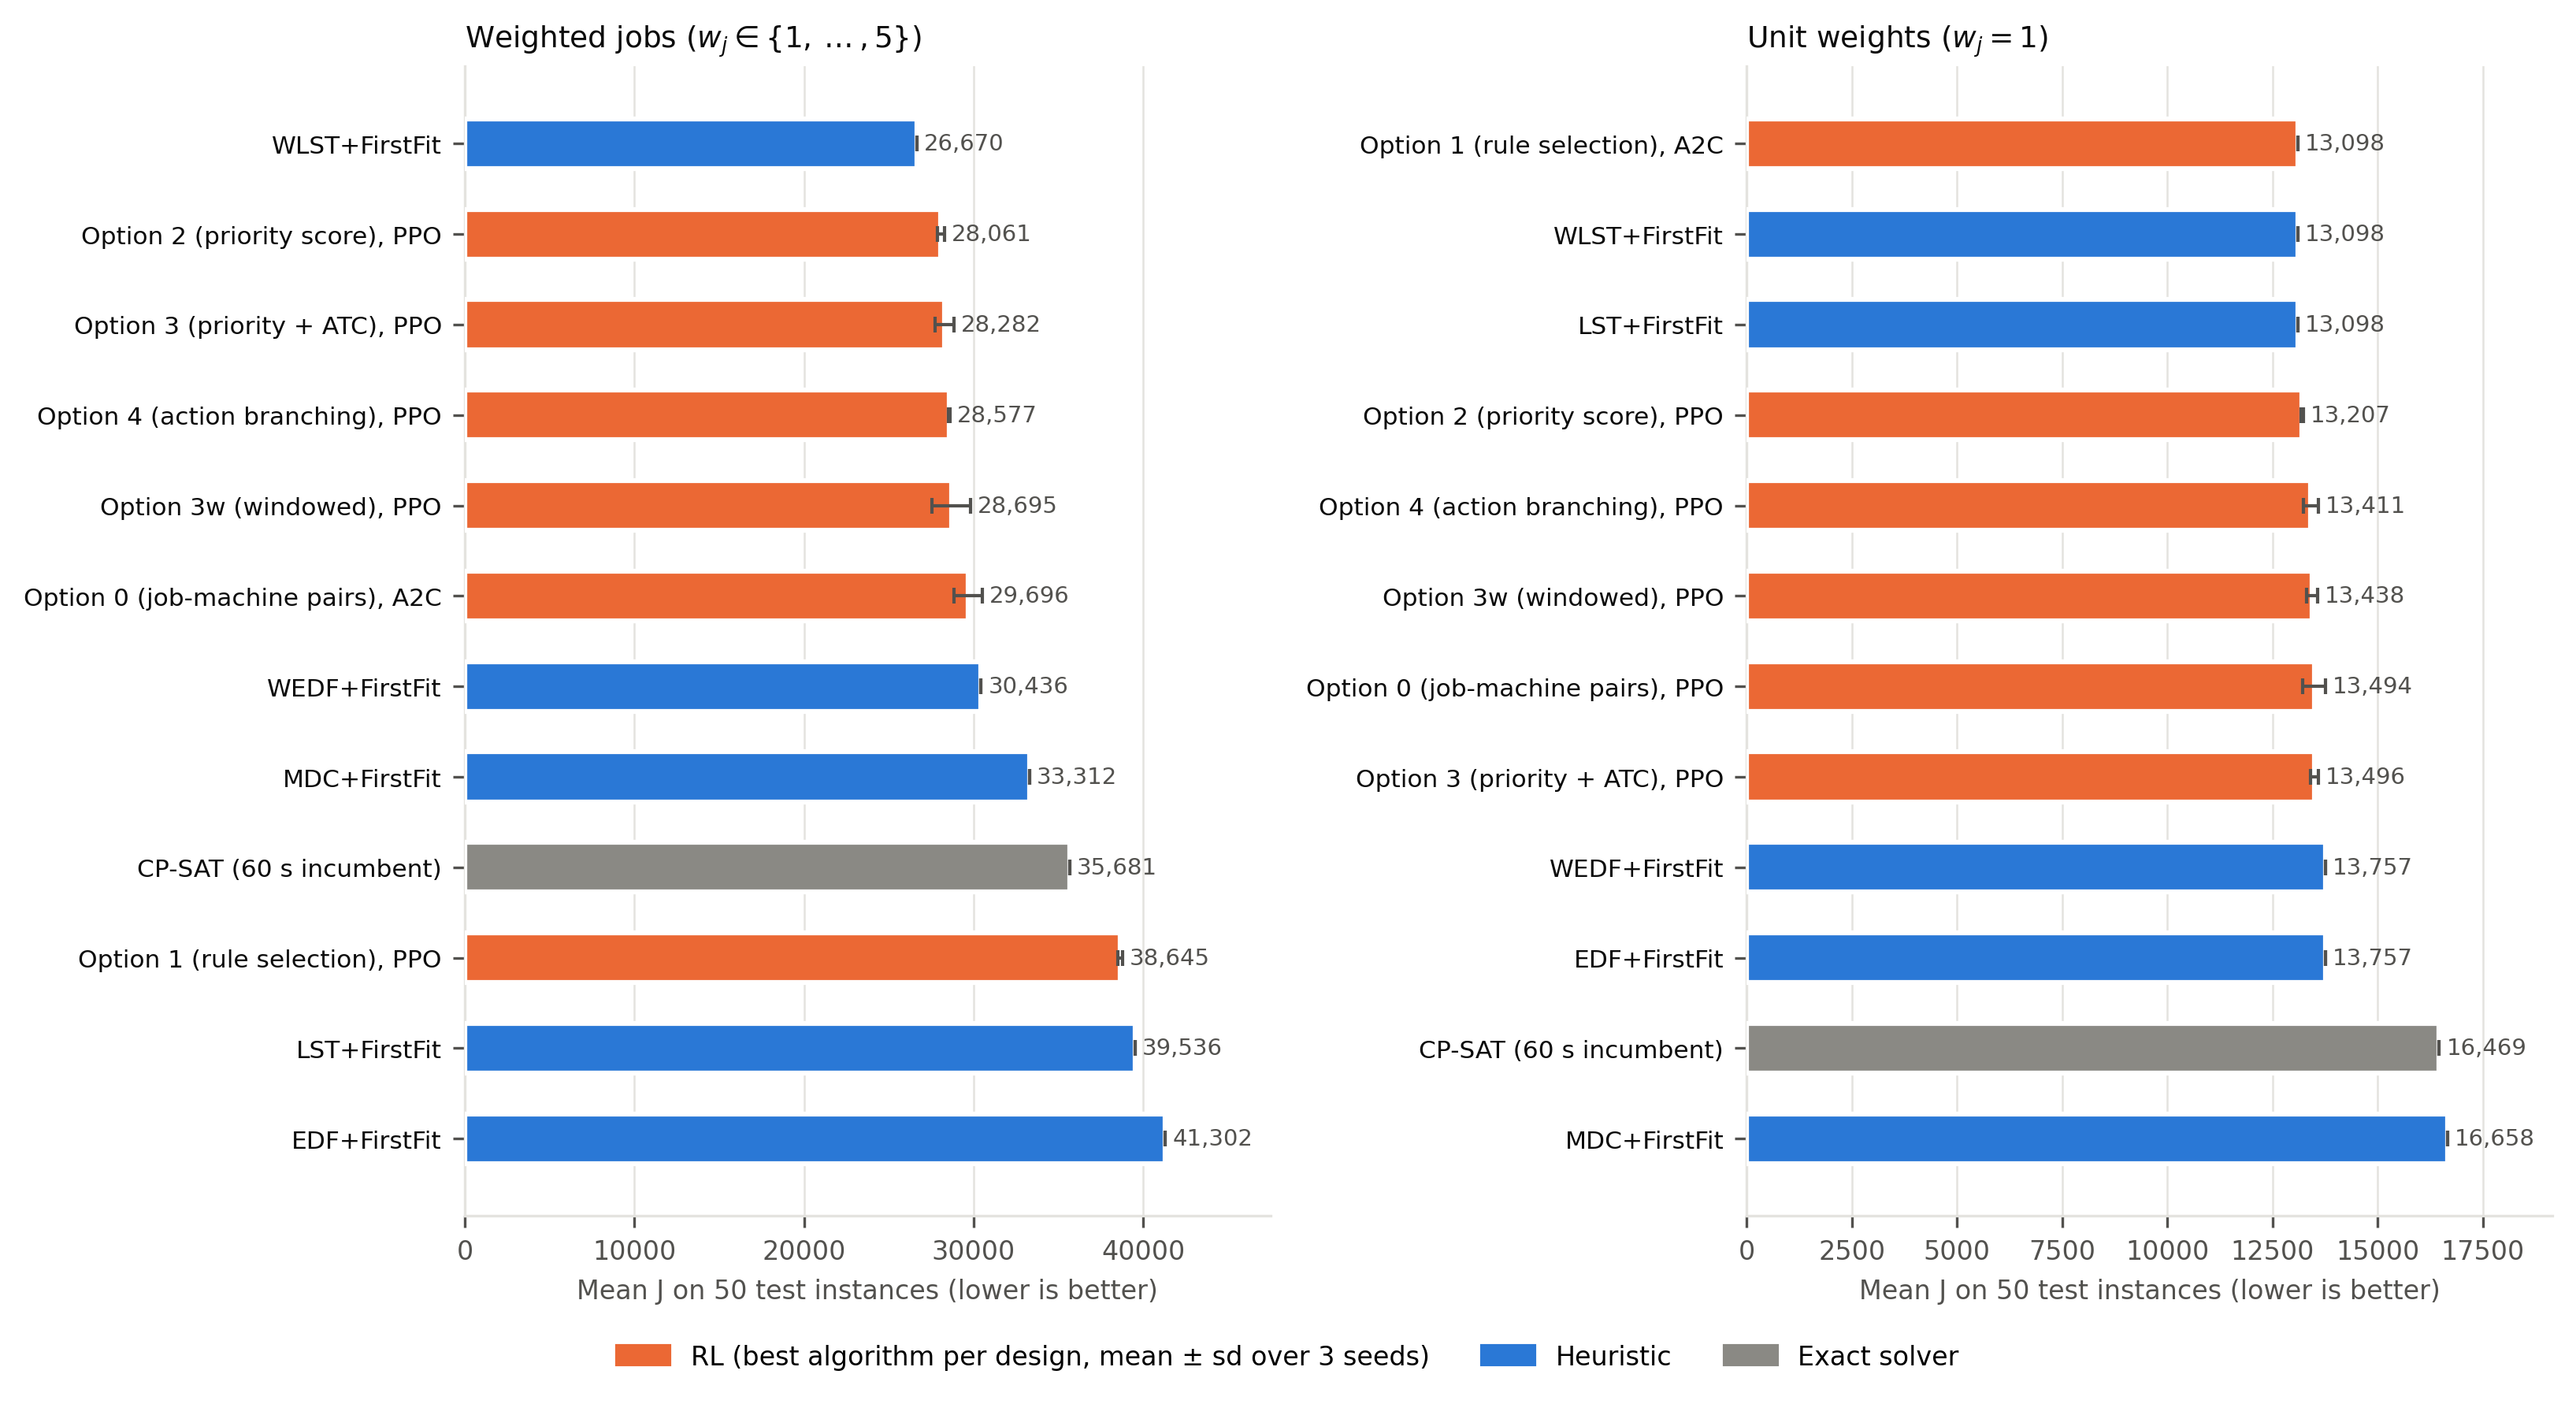
\includegraphics[width=\linewidth]{Images/v2_offline_designs.png}
\caption{Offline results: the best final agent of each design (orange, mean $\pm$ s.d.\ over 3 seeds) against the leading heuristics (blue) and CP-SAT's 60-second schedule (grey). Left: weighted jobs; right: unit weights.}
\label{fig:offline}
\end{figure}

\subsection{Combined Objectives}\label{sec:res-mo}
\Cref{fig:regime} answers the entire research question in one view. For each objective and setting, it compares the best-performing RL agent with the best heuristic. Offline with weighted jobs is the only setting where we see RL win. Note that the multipliers indicate the weight of the added term relative to a reference value. At $\times 1$, the added term is worth as much as $J$ on the best heuristic's schedule; at $\times 4$, it is worth four times as much, so it dominates the objective.

\begin{figure}[htbp]
\centering
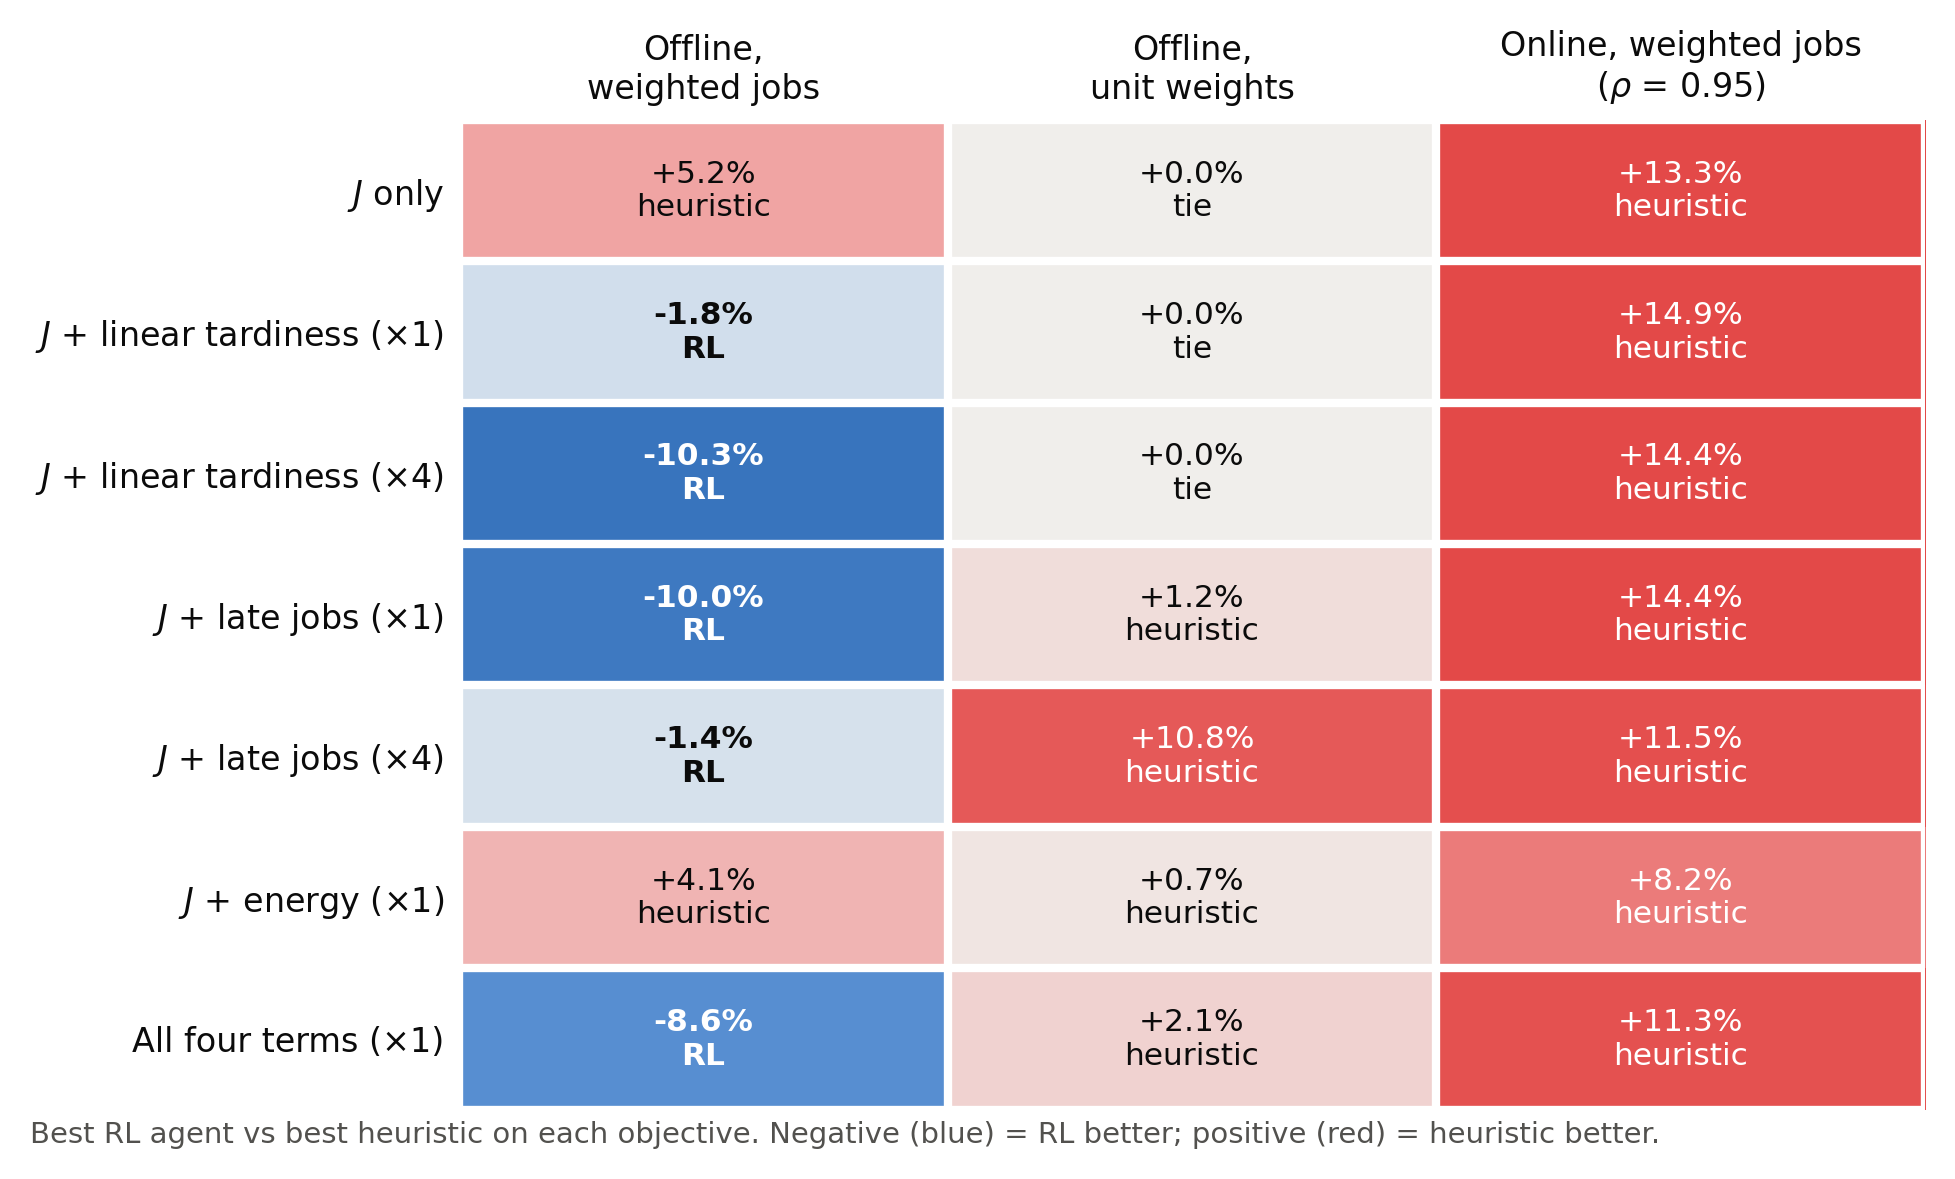
\includegraphics[width=0.85\linewidth]{Images/v2_regime_grid.png}
\caption{Best RL agent against the best heuristic on each objective (rows) and setting (columns); blue means RL is better, red means the heuristic is better. Weights are multiples of the reference values, which make each added term equal to $J$ on the best heuristic's schedule. Only RL agents with at least two evaluated seeds are included.}
\label{fig:regime}
\end{figure}

\subsection{Online Training Budget}\label{sec:res-online}
Whilst training multiple RL models, it was found that most of the online gap, especially for Option 2, would fall as training steps increased. Option 2's mean $J$ falls from $39{,}947$ at 300k steps to $26{,}515$ at 1M (+21\% over EDF+Consolidate) and $24{,}921$ at 2M (+13\%, 2 seeds), and its best 1M seed is within 4.3\% of the heuristic. Option 0 improves on average but remains 55\% behind at 1M. Online A2C did not learn: Option 0 A2C produced the same schedule as FCFS+FirstFit ($J = 44{,}920$) on all three seeds.

\subsection{Other Findings}\label{sec:res-other}
\paragraph{Action-space design.} Learning with job priority (Options 2 and 3) worked best in every setting. Picking job-machine pairs directly (Option 0) was 6\% worse offline and remained 55\% behind online at 1M steps. Choosing job and machine with two heads (Option 4) was competitive offline, but failed online. Rule selection (Option 1) would mostly collapse onto a single rule, often reproducing LST exactly.

\paragraph{Training stability.} In 8 independent offline runs of the same Option 2 configuration (default hyperparameters, 300k steps), one diverged ($J = 69{,}367$, against $28{,}352$--$30{,}925$ for the other seven). Online seeds differed much more: Option 2 at 300k steps ranged from $30{,}076$ to $53{,}231$.

\paragraph{Energy.} Interestingly, energy was the only metric on which RL never beat the best heuristic in any scenario. Training with the energy term had no diverging runs, but it did not make training meaningfully more stable either; it only traded $J$ for lower energy.

\paragraph{No single heuristic wins.} The best rule often changes depending on deadline tightness and load: EDF with loose offline deadlines, WLST with medium and tight deadlines, LST with unit weights, and Consolidate placement was the best at every online load.

\paragraph{Hyperparameter tuning.} The library defaults were the best configuration in 8 of the 24 RL studies.

\section{Discussion}\label{sec:discussion}
\paragraph{When does RL beat heuristics?} Our results suggest three conclusions. First, \emph{the objective must not be one that a simple rule solves well}. RL never improved on the best heuristic in simple cases (Option 1 can only reproduce a rule): with unit weights and squared tardiness, LST matched every proven optimum of the CP-SAT exact solver on small instances. When the objective mixes metrics, no single heuristic is designed for that combination, and this is where we saw our only RL wins. Heuristics are designed for a specific problem and solve it efficiently and effectively. Second, \emph{RL only outperforms when jobs have weights}. Weights give a learned priority more to work with; notably, online only considered weighted jobs due to a lack of training time. Future RL work could combine different metrics into learned job weights to simplify the agent's task. Third, \emph{the agent must be trained enough for the scenario}. Offline had the most data due to its much faster training times, and 1M steps offline came within 5\% of the best heuristic. Online, 300k steps left RL 70\% behind, and 1--2M steps slowly closed the gap for the best designs.

\paragraph{Multi-objective results.} At moderate weights, the agents that performed best on the composite objectives were, somewhat surprisingly, those trained solely on squared tardiness. Their schedules simply happened to produce fewer late jobs and lower linear tardiness, making this behaviour a by-product of how the RL policy structures schedules rather than evidence of targeted learning. This cautions against over-interpreting improvements in metrics that were not explicitly optimised. One would normally expect agents trained with explicit composite objectives to do best on those same objectives, yet this did not occur, possibly because they were trained for only 300,000 steps with default hyperparameters, against 1M tuned steps for the $J$-only agents. At higher weights, however, the agents trained on the composite objective began to dominate, indicating genuine learning aligned with the intended optimisation.

\paragraph{Online difficulty.} Online results depend heavily on the random sequence of job arrivals, which the agent cannot predict, so the training signal is much noisier than offline \cite{mao2019variance}. To reduce this noise, the critic (but not the policy) was given a summary of jobs that had not yet arrived. Because only the critic sees this information, the policy's learning signal stays unbiased \cite{mao2019variance, pinto2018asymmetric}, but online RL still remained well behind the best heuristic. Online episodes are also about ten times longer than offline, and the agent must observe over a thousand job slots, so training was slower and far less stable. Several other changes were tested without closing the gap, including potential-based reward shaping \cite{ng1999shaping}, a capacity look-ahead, reward scaling and undiscounted returns ($\gamma = 1$). The one change that clearly helped was more training.

\paragraph{Practical considerations.} RL is costly to build and to train. Training was unstable, and a single online tuning trial took four to five hours. Beyond compute, RL is expensive to model: reaching the current results took around three months of iterating on the reward, action space, observation and training, and RL still does not beat the best heuristic in most settings. Heuristics, by contrast, need no training, give the same schedule every time, are cheap to run, and are easy to explain. For a cloud provider, a well-chosen heuristic is therefore the practical default, and RL is worth its cost mainly where the objective combines several goals, jobs differ in importance, and enough compute is available.

\paragraph{Limitations.} All instances are synthetic and of one size (100 jobs, 10 machines, 4 resources), and results use 3 seeds. Real traces should be examined to get concrete results, along with more training.

\section{Conclusion}\label{sec:conclusion}
This project formulated cloud resource allocation as a multi-resource scheduling problem, built offline and online environments, and compared six RL action-space designs, trained with PPO and A2C, against 49 heuristics and an exact solver. On the main objective, weighted squared tardiness, RL came within 5\% of the best heuristic offline. When considering multiple objectives, RL did beat the best heuristic by 2--10\% for a few metric combinations, but notably the best RL models for some of these combinations were those trained without the added terms in their objective. Online, RL didn't manage to beat the best heuristic; however, the data indicates it could be a computational issue: as training steps increased, so did RL performance, but larger models and robust testing of them did not fit within the project timeline. Learning a job priority was the most effective design, although getting RL to train reliably required very careful diagnosis and refinement. RL could be a competitive algorithm for cloud resource allocation, especially with multiple objectives, but this report found that a simple heuristic remains the best choice, especially considering computational and modelling resources.

\section{Future Work}
The following topics were only touched on briefly in this report and are directions for future research.
\begin{itemize}
    \item \textbf{The online case.} RL was trained online at a single load ($\rho = 0.95$) with weighted jobs. Future work should train for longer and with more seeds, cover the other loads and a unit-weight online setting, and test generalisation across loads and deadlines (in progress).
    \item \textbf{Idling and capacity reservation.} Agents were free to idle, but whether they actually learned to reserve capacity for future jobs was not analysed.
    \item \textbf{Training stability.} The causes of divergence and seed variance, and larger tuning budgets, were not studied in depth.
    \item \textbf{Action spaces and architectures.} Why rule selection collapsed and the two-headed design failed online; graph neural network encoders \cite{gnn2024jsspsurvey}, large discrete action-space methods \cite{dulacarnold2015largeactionspaces}, branching \cite{tavakoli2018actionbranching} and hybrid architectures \cite{ml_ra_litrev2025}; and learned placement to close the energy gap.
    \item \textbf{Alternative formulations.} RCPO and PPO-Lagrangian under the final objective, and smaller formulation choices such as the offline limit of one job start per time step.
    \item \textbf{Objectives and metrics.} Composite-objective agents with the full training setup (in progress), a single agent conditioned on the objective weights, and other metrics such as response time.
    \item \textbf{Realism and scale.} Real traces such as the Google cluster trace \cite{reiss2012googletrace} or Azure \cite{cortez2017resourcecentral}, and larger clusters.
    \item \textbf{Heuristic discovery.} Extracting interpretable rules from the learned priorities.
\end{itemize}

\section*{Data Management Plan}
All code, raw results (per-instance metrics for every method and seed), processed tables and figures, Optuna study logs and the chronological experiment log are in the public GitHub repository\footnote{\url{https://github.com/Ethan-Ty-Riekert/Neural-Knapsack-Research-Project}}. Results are under \texttt{Results/} (raw runs, tuning studies, and the processed \texttt{ALL\_RESULTS} archive), and every number in this report can be regenerated from them with the scripts provided. All instances are synthetic and generated from fixed random seeds, so no personal or sensitive data is involved. Trained model files are regenerated by the training scripts and are not version-controlled. The version cited in this report is a tagged release on the \texttt{main} branch.

\section*{Generative AI Use Statement}
Claude Code (Anthropic) was used as a coding and research assistant throughout this project. The original environment and the translation of the mathematical formulation into code were done by hand. Claude Code was used in the following ways:
\begin{itemize}
    \item \textbf{Implementation and experiments.} Implementing models, training and evaluation code, and running experiments from a queue. Every result was reviewed personally.
    \item \textbf{Literature search.} Finding relevant papers and resources. Every source cited in this report was checked by the author.
    \item \textbf{Modelling discussions.} Discussing modelling ideas and design choices against the literature, and giving a second opinion on decisions such as reward design, action spaces and evaluation protocols. Every modelling decision was made and approved by the author.
    \item \textbf{Diagnostics.} Investigating unexpected results and training failures, and checking them against the literature.
    \item \textbf{Report review and editing.} Reviewing the report for consistency with the code and the latest results, checking numbers, claims and citations, and helping to edit the text. All content was reviewed and approved by the author.
\end{itemize}
Claude worked under a fixed set of rules: every design decision had to be cited and justified, or derived; implementation and discussion had to remain mathematically grounded; and every decision and result had to be recorded in an experiment log. Separate Claude agents were also used weekly to check the code's efficiency, mathematical rigour and factual accuracy. Using Claude allowed far more experiments, analyses and model iterations than would otherwise have been possible.

\newpage
\bibliographystyle{IEEEtran}
\bibliography{references}

\newpage
\appendix
\section{Nomenclature}\label{sec:AppendixA}
\begin{table}[htbp]
\centering
\caption{Nomenclature}
\label{tab:nomenclature}
\begin{tabular}{ll}
\toprule
\multicolumn{2}{l}{\textbf{Sets}}\\
\midrule
$J$ & Set of jobs, indexed by $j$ \\
$J_t$ & Jobs waiting (arrived, not yet started) at time $t$ \\
$P_t$ & Jobs processing (started, not finished) at time $t$ \\
$M$ & Set of machines, indexed by $m$ \\
$R$ & Set of resource types, indexed by $r$ \\
$\mathcal{T}$ & Set of discrete time periods, indexed by $t$ \\
\midrule
\multicolumn{2}{l}{\textbf{Parameters}}\\
\midrule
$p_j$ & Processing duration of job $j$ \\
$a_{jr}$ & Requirement of job $j$ for resource $r$ \\
$C_r$ & Capacity of each machine for resource $r$ \\
$H$ & Length of the planning horizon \\
$d_j$ & Due date of job $j$ \\
$w_j$ & Priority weight of job $j$ \\
$\tau_j$ & Arrival time of job $j$ ($0$ offline) \\
$\nu$, $\rho$ & Arrival rate and load factor (online) \\
TF, RDD & Tardiness factor and due-date range (offline deadlines) \\
$\lambda_1, \lambda_2, \lambda_3$ & Weights in the initial objective \cref{eq:objective-v1} \\
$\lambda_T, \lambda_U, \lambda_E$ & Weights in the final objective \cref{eq:objective-v2} \\
\midrule
\multicolumn{2}{l}{\textbf{Decision variables}}\\
\midrule
$x_{jmt}$ & 1 if job $j$ starts on machine $m$ at time $t$; 0 otherwise \\
$y_m$ & 1 if machine $m$ is used; 0 otherwise \\
$s_j$ & Start time of job $j$ \\
$T_j$ & Tardiness of job $j$, $\max(0, s_j + p_j - d_j)$ \\
$U_j$ & 1 if job $j$ finishes after $d_j$; 0 otherwise \\
$E$ & Energy: total active machine-time \\
$U_{mrt}$ & Total usage of resource $r$ on machine $m$ at time $t$ \\
$\theta$ & Peak utilisation ratio, $\max_{m,r,t} U_{mrt}/C_r$ \\
\bottomrule
\end{tabular}
\end{table}

\section{Constraints}\label{sec:AppendixB}
Let $\mathcal{T} = \{0, 1, \dots, \bar{H}\}$, where $\bar{H}$ is any upper bound on the time to finish all jobs (e.g.\ $H + \sum_j p_j$, under the extended horizon). For each job, let $\mathcal{T}_j = \{t \in \mathcal{T} : \tau_j \le t \le \bar{H} - p_j\}$ be its feasible start times.

\paragraph{Assignment.} Each job starts exactly once, on exactly one machine, and never before it arrives:
\begin{equation}\label{con:assign}
    \sum_{m \in M} \sum_{t \in \mathcal{T}_j} x_{jmt} = 1, \qquad \forall j \in J.
\end{equation}
\paragraph{Offline start rate.} Offline, at most one job starts per time step:
\begin{equation}\label{con:one-start}
    \sum_{j \in J} \sum_{m \in M} x_{jmt} \le 1, \qquad \forall t \in \mathcal{T}.
\end{equation}
\paragraph{Machine activation.} A job can only be placed on an active machine:
\begin{equation}\label{con:machine-use}
    x_{jmt} \le y_m, \qquad \forall j \in J,\ m \in M,\ t \in \mathcal{T}_j.
\end{equation}
\paragraph{Start time.}
\begin{equation}\label{con:start-time}
    s_j = \sum_{m \in M} \sum_{t \in \mathcal{T}_j} t\, x_{jmt}, \qquad \forall j \in J.
\end{equation}
\paragraph{Resource usage and capacity.} A job started at $t'$ occupies its resources during $[t', t'+p_j)$, so the usage at time $t$ counts every job started within the previous $p_j$ steps. Usage may never exceed capacity:
\begin{equation}\label{con:resource-usage}
    U_{mrt} = \sum_{j \in J} \; \sum_{\substack{t' \in \mathcal{T}_j \\ t - p_j < t' \le t}} a_{jr}\, x_{jmt'} \;\le\; C_r, \qquad \forall m \in M,\ r \in R,\ t \in \mathcal{T}.
\end{equation}
\paragraph{Tardiness, late jobs and peak utilisation.}
\begin{equation}\label{con:tardiness}
    T_j \ge s_j + p_j - d_j, \quad T_j \ge 0, \quad T_j \le \bar{H}\, U_j, \qquad \forall j \in J,
\end{equation}
\begin{equation}\label{con:theta}
    \theta \ge \frac{U_{mrt}}{C_r}, \qquad \forall m \in M,\ r \in R,\ t \in \mathcal{T}.
\end{equation}
Because the objectives are minimised and increase with $T_j$, $U_j$ and $\theta$, these inequalities hold with equality at the optimum. Finally, $x_{jmt}, y_m, U_j \in \{0, 1\}$.

\section{Hyperparameter Search Space}\label{sec:AppendixC}
\begin{table}[htbp]
\centering
\caption{Hyperparameters searched by Optuna (ranges after \cite{andrychowicz2021onpolicy}). ``log'' means sampled log-uniformly; lists are categorical choices. Trial 0 of every study used the library defaults instead.}
\label{tab:hp}
\begin{tabular}{lll}
\toprule
Hyperparameter & PPO & A2C \\
\midrule
Learning rate & $3\times10^{-5}$ -- $10^{-3}$ (log) & $10^{-4}$ -- $3\times10^{-3}$ (log) \\
Rollout length (all 4 environments) & 2048, 4096, 8192, 16384 & 20, 80, 320 \\
Minibatch size & 64, 256, 1024 & -- \\
Epochs per update & 3, 5, 10 & -- \\
Discount factor $\gamma$ & 0.99, 0.995, 0.999 & 0.99, 0.995, 0.999 \\
GAE $\lambda$ & 0.9, 0.95, 0.98 & 0.9, 0.95, 1.0 \\
Clip range & 0.1, 0.2, 0.3 & -- \\
Entropy coefficient & $10^{-4}$ -- $3\times10^{-2}$ (log) & $10^{-4}$ -- $3\times10^{-2}$ (log) \\
\bottomrule
\end{tabular}
\end{table}

\section{Experimental Details}\label{sec:AppendixD}
\paragraph{Offline deadlines.} Following Potts and Van Wassenhove \cite{potts1985wtardiness}, each $d_j$ is drawn uniformly from $[\,\bar{C}(1 - \mathrm{TF} - \mathrm{RDD}/2),\ \bar{C}(1 - \mathrm{TF} + \mathrm{RDD}/2)\,]$ and is at least $p_j$. Here $\bar{C}$ is a lower bound on the time to finish all jobs (the larger of the number of jobs, since one job starts per step, and the total work divided by the cluster's capacity), TF is the tardiness factor and RDD $= 0.6$ the range of due dates, which sets how spread out deadlines are.

\paragraph{Online deadlines and job sizes.} A job's deadline is its arrival time plus a slack drawn uniformly from $\{10, \dots, 60\}$ time steps ($\{5, \dots, 25\}$ in a tight-deadline variant). Durations and demands are log-normal, not Gaussian: the logarithm of the size is normally distributed (with $\sigma = 1$), giving many small jobs and a few large ones. The location parameter is set so that the mean equals that of the offline uniform distribution, and sizes are capped at four times the offline maximum (durations of at most 40 steps).

\paragraph{Tuning protocol.} Each of the 24 studies ran 12 trials of 300,000 steps with 4 parallel environments; trial 0 used the Stable-Baselines3 defaults, which lie outside the log-scaled search space (the default entropy coefficient is 0). Every 75,000 steps, a trial reported its mean $J$ on 5 validation instances. Optuna's median pruner stopped the trial if this was worse than the median of the values earlier trials had reported at the same step; pruning only starts after 5 trials have finished. A completed trial's score is its mean $J$ on all 20 validation instances, and the best score gives the study's single chosen configuration. The offline configuration was reused for the unit-weight setting. Three online PPO studies (Options 0, 2 and 4) trained at about 20 steps per second, roughly 4--5 hours per trial, and were stopped after 3--7 trials to meet the project deadline; the best completed trial was used as usual. The defaults were the best configuration in 8 of the 24 studies.

\paragraph{Faults fixed in the final training version.} Each fault was measured directly in training logs.
\begin{enumerate}[nosep]
    \item \emph{The critic did not learn.} Squared-tardiness returns are in the hundreds to thousands, and the value and policy losses share one clipped gradient, so the value error swamped each update. The critic explained none of the variance in returns, and A2C policies stayed close to uniformly random. Rewards are now divided by a running estimate of the standard deviation of the return \cite{engstrom2020implementation, andrychowicz2021onpolicy}; afterwards the critic explained 30--99.9\% of the variance.
    \item \emph{Deterministic evaluation idled.} Idle is a single action, while the probability of starting a job is split across many (job, machine) actions. For an undecided policy, idle could be the single most likely action in every state, so a ``most likely action'' rule idled indefinitely even though the trained (sampling) policy placed jobs 98\% of the time. The two-stage rule of \cref{sec:evaluation} fixes this, and is identical to the most-likely-action rule for confident policies.
    \item \emph{Idling could repeat forever.} An idle used to advance time by one step and return the agent to an unchanged decision. Event-driven idling advances to the next arrival or completion instead. Waiting between events never helps, since a job that fits at an intermediate step also fits now and finishes earlier, so no schedule is lost.
\end{enumerate}
Together, these changes reduced offline Option 0 A2C's validation $J$ from 234,116 to 43,164.

\end{document}
